\begin{figure}[htbp]
  \centering
  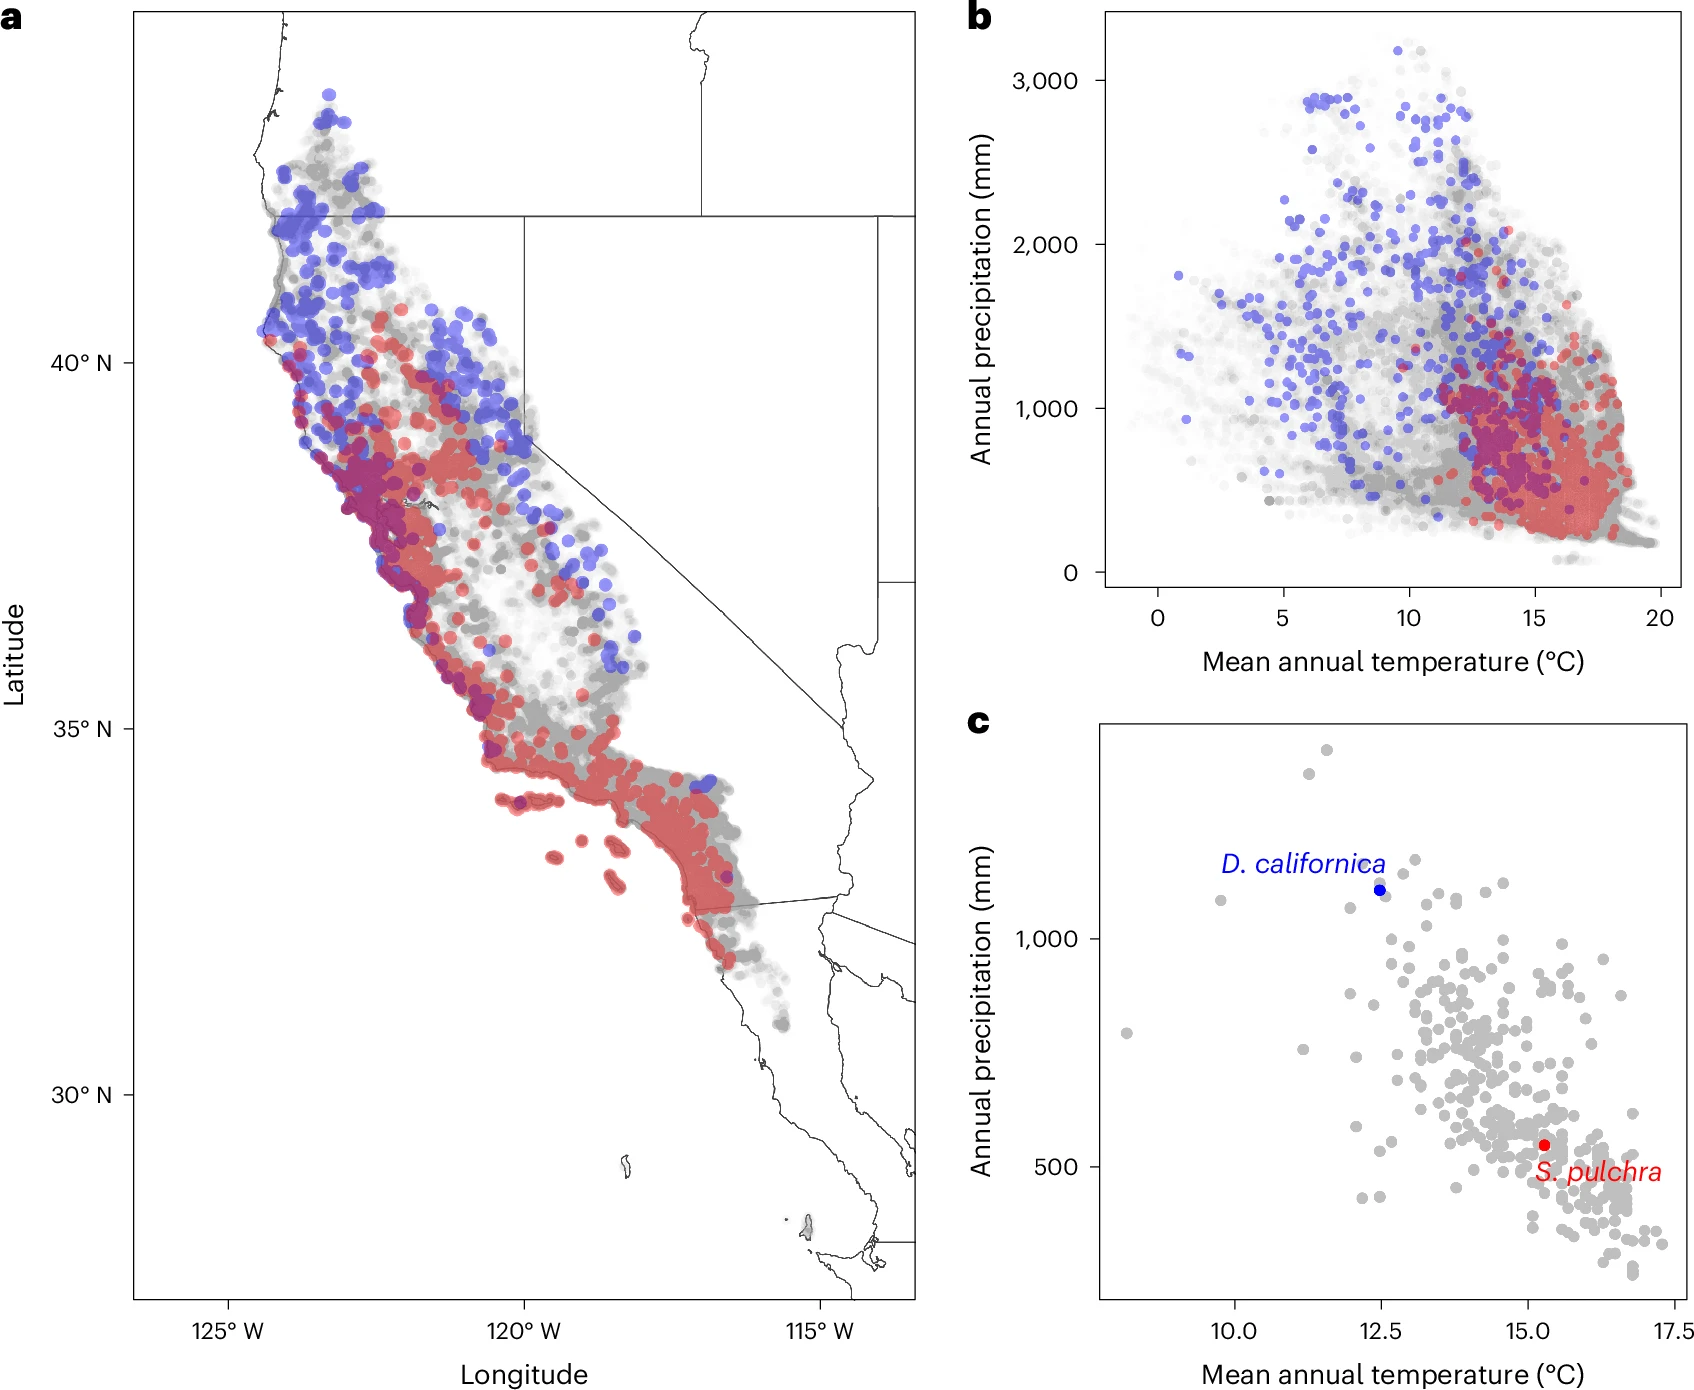
\includegraphics[width=0.9\linewidth]{../figures/grassland.png}
  \caption{\textbf{Grassland species occur along geographic and climatic gradients to estimate niches.}. a, Occurrence of grassland species in the CFP, retrieved from the GBIF data (grey points), highlighting two example species, \textit{D. californica} in the north (blue points) and \textit{S. pulchra} in the south (red points). b, Species occurrence in climate space of mean annual temperature and annual precipitation, retrieved from the CHELSA data (grey), highlighting the same two example species, \textit{D. californica} under cool and wet climates (blue) and \textit{S. pulchra} under warm and dry climates (red). c, Estimated climatic niche centroids from the medians of temperature and precipitation for each species (grey), highlighting the two species (blue and red).}
  \label{fig:grassland}
\end{figure}
